This section will discuss different concepts of a Random Forest (RF) algorithm, starting with the basis of the RF:\@ decision tree. Decision tree is an algorithm that generates a tree graph of decisions based on the input provided and their possible outcomes, and as a consequence, it partitions the input space into multiple regions, with each region accounting for a different outcome~\cite{murphyML}. An example of a simple decision tree based on two inputs is shown in figure~\ref{fig:decisionTree}. 

The most significant advantage of the decision tree, and subsequently, random forest algorithm, is that it is relatively simple, explainable, easy to train and interpolate with little computational resources. However, one crucial drawback of a decision tree is its instability: minor data changes might affect the tree structure, making the decision tree a high variance estimators~\cite{murphyML}. Attempts have been made to reduce the uncertainty of the decision tree, one of which is the so-called Random Forest algorithm, which Breiman proposed in 2001~\cite{BreimanRF}. RF made up for the high variance of a single decision tree by averaging the results over a ``forest'' of decision trees, with each tree representing an independent sampled vector. The concept of decision tree and RF, therefore, fit within the scope of the calibration problem.

\subsection{Training and evaluation method for supervised models}  

500 DEM simulations with randomized combinations of input parameters have been performed to train the NN and RF model, which will help create a database that maps DEM microparameters to static AoR. The other 125 simulations did not finish on the time constraint set and, as a result, were marked as an inaccurate combination. 

\begin{figure}[H]
    \centering
    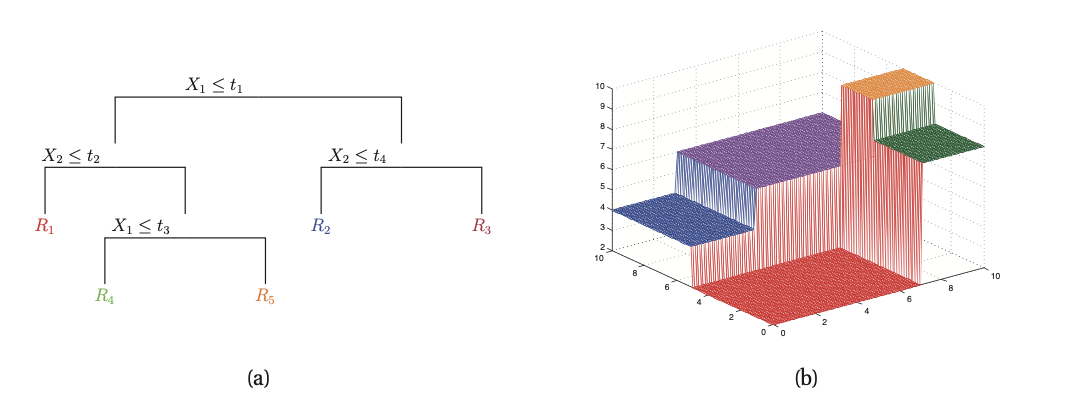
\includegraphics[scale=0.8]{regressionTree.png}
    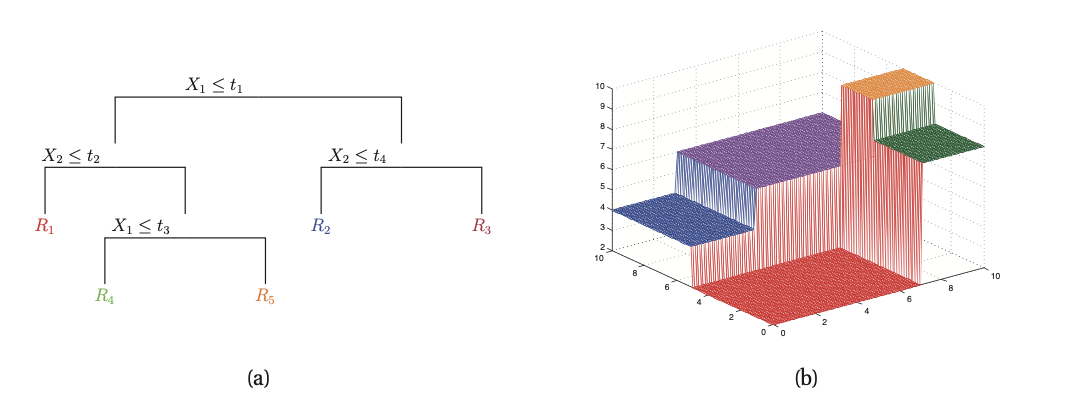
\includegraphics[scale=0.8]{decisionTree.png}
    \caption{Example of a decision tree regressor on a two-input problem~\cite{murphyML}.}\label{fig:decisionTree}
\end{figure}




